\section{Evaluation}
\label{sec:eval}

In this section, we evaluate the graph summarisation under three different aspects:
\begin{description}
	\item[Performance] the amount of computational power needed by the implementation of a \gls{summarisation-relation} for generating a summary;
	\item[Compression] the ability of the graph summarisation to reduce the number of nodes and edges needed for describing the graph's structure; and
	\item[Precision] the precision of a generated graph summary with regards to the original graph, as measured by the \gls{precision}.
\end{description}
We present those three dimensions of the evaluation in Section~\ref{sec:eval:design}.
In order to give ground to the study of the graph summarisation under those three dimensions, we consider a collection of 14 datasets described in Section~\ref{sec:eval:datasets} of varying size and complexity. The size of a graph to summarise will impact on the performance and compression of a summarisation implementation, while the complexity in terms of vocabulary (i.e., the use of \gls{types} and \gls{attributes} and combinations thereof) will manifest itself on the precision of a summary.\\

In this evaluation, we consider the following parameters:
\begin{itemize}
	\item we want to summarise a graph $G=\left\langle V, A, l_V \right\rangle$;
	\item the result of summarising the graph $G$ is the summary graph $\mathcal{S} = \left\langle \mathcal{W}, \mathcal{B}, l_{\mathcal{W}} \right\rangle$ according to the summarisation relation $R$;
	\item with regards to the classification in Section~\ref{sec:error-classification}, we measure the error in the created summary by comparing it to the bisimulation summary \glssymbol{fbt-bisimulation-summary} of $G$, i.e., $\glssymbol{fbt-bisimulation-summary} = \left\langle \mathcal{W}_{fbt}, \mathcal{B}_{fbt}, l_{\mathcal{W}_{fbt}} \right\rangle$ according to the summarisation relation $R_{fbt}$; and
	\item The bisimulation \gls{summarisation-relation} described in Section~\ref{chap:summary:bisim} maps nodes of the graph to a same sumnode if they all share the same outgoing and incoming paths. The bisimulation summarisation relation is smaller with regards to the partial order \glssymbol{partial-order} than any of the approximate graph summarisation presented in Section~\ref{sec:approximate} since its summarisation relation is more restrictive. Therefore, we assume the existence of a relation $S \subseteq \mathcal{W}_{fbt} \times \mathcal{W}$ that maps the bisimulation summary to a summary generated from the summarisation relation $R$, i.e., such that $R_{fbt} \sqsubseteq R$.
\end{itemize}

\subsection{Design}
\label{sec:eval:design}

We describe in this section the design of the evaluation. We first present the environment of our experimental framework. Then, we describe the dimensions of our evaluation.

\subsubsection{Environment}

The bisimulation summary \glssymbol{fbt-bisimulation-summary} presented in Section~\ref{chap:summary:bisim} is the most precise summary of the entity graph, since all incoming and outgoing (and combination of) paths in the summary do exist in the entity graph $G$. In this evaluation, we use as the \emph{gold standard} summary of an entity graph the \gls{ft-bisimulation-summary} instead of the \gls{fbt-bisimulation-summary} for performance reason. This gold standard summary ensures that all outgoing paths do exist. The presented \glspl{summarisation-relation} have been implemented using the Hadoop\footnote{Hadoop: \url{http://hadoop.apache.org/}} MapReduce framework according to the algorithm outlined in Section~\ref{sec:mapreduce}.
% Our Hadoop cluster is composed of 10 machines.

\subsubsection{Evaluation Dimensions}

We present in this section three dimensions we use for evaluating a summary, i.e., the summary \emph{compression}, the computational \emph{performance} of the \gls{summarisation-relation}, and the \emph{precision} of the summary.

\begin{quotation}
	\item[\emph{Summary compression.}]

	A summary is smaller if its size $\vert \mathcal{B} \vert$ (number of sumedges) and its order $\vert \mathcal{W} \vert$ (number of sumnodes) are inferior to the size $\vert A \vert$ and the order $\vert V \vert$ of the graph it was created from.

	Apart from the \gls{unique-type-summary} $R_{ut}$, the presented \glspl{summarisation-relation} in Section~\ref{sec:approximate} create a summary which is always smaller or equal to the graph, since there is a one-to-one mapping from the entity graph to the summary.

	The \emph{unique type} summarisation relation $R_{ut}$ may assign several sumnode to a same node $u \in V$ when the set of \gls{types} is greater than one, i.e., when $\vert types(u) \vert > 1$. The order of a \gls{unique-type-summary} $\mathcal{S}_{ut} = \left\langle \mathcal{W}_{ut}, \mathcal{B}_{ut}, l_{\mathcal{W}_{ut}} \right\rangle$ is at most equal to the number of types in the graph, i.e., $\vert \mathcal{W}_{ut} \vert = \vert \{ l_{\mathcal{W}_{ut}}(c) \mid \forall (u, c) \in V^2_{ut}\; (u, \glssymbol{atype}, c) \in \mathcal{B}_{ut} \wedge \glssymbol{atype} in T \} \vert$. However, in the worst case, its size can equal $\vert \mathcal{B}_{ut} \vert = \vert \mathcal{W}_{ut} \vert ^d$, with $d$ being the diameter\footnote{The diameter $d$ of a graph $G$ is the maximum distance between any two nodes of the graph. The distance between two nodes is the number of edges in the shortest path that connects the two.} of the entity graph. Indeed, every node of the graph can be associated with every types. Therefore when applying the \emph{unique type} summarisation relation $R_{ut}$ over such a graph, we need for each path in $G$ to create an edge to each type for every node of the path. Figure~\ref{fig:unique-type-summary-size} depicts the size of the \gls{unique-type-summary} in the worst case scenario, where all nodes are both of types $A$ and $B$.

	The summary is sensitive to heterogeneous entity graph. Indeed, there can be as many sumnodes in an \gls{attributes-summary} $\mathcal{S}_a = \left\langle \mathcal{W}_{a}, \mathcal{B}_{a}, l_{\mathcal{W}_{a}} \right\rangle$ as there is elements in the attribute powerset minus the empty set, i.e., $\vert \mathcal{W}_a \vert = \vert \mathbb{P} \left( \{ \alpha \mid \forall (u, v) \in \mathcal{W}_a\; (u, \alpha, v) \in \mathcal{W}_a \} \right) \vert - 1$. Such an order of the summary can be expected for any summarisation relation based on the set of \gls{attributes}, i.e., the summarisation relations $R_{at}$, $R_{ioa}$, $R_{ioat}$, and $R_{fbt}$.\\

	We measure the amount of information from a given graph $G_1 = \left\langle V_1, A_1, l_{V_1} \right\rangle$ that is compressed into another graph $G_2 = \left\langle V_2, A_2, l_{V_2} \right\rangle$. To this end, we compare the size and order of $G_2$ against the size and order of $G_1$. We report this comparison as the ratio $G_2:G_1$:

	$$
	G_2:G_1 = \frac{\vert V_2 \vert + \vert A_2 \vert}{\vert V_1 \vert + \vert A_1 \vert}
	$$

	\item[\emph{Algorithm performance.}]

	%The MapReduce implementation of the graph summarisation is composed of two separate steps:
	%\begin{inparaenum}[(1)]
	%\item a \emph{mapping} step, where we assign a node of the entity graph to its $\sim$-equivalence class; and
	%\item a \emph{edges} step, where we compute the edges of $G^\sim$.
	%\end{inparaenum}
	We evaluate the computational performance of a \gls{summarisation-relation} by analysing the CPU time\footnote{The accumulated CPU time as reported with the \texttt{CPU\_MILLISECONDS} counter of Hadoop.} on the \hyperref[step-he]{Step 3} of the graph summary computation, as described in Section~\ref{chap03:algo:edge-materialisation} for the MapReduce case. We do not report on the \hyperref[step-hn]{Step 2} because the evaluated \glspl{summarisation-relation} have the same complexity, achieving similar times on this step.

	\item[\emph{Summary precision.}]

	With regards to all three classification of errors, we evaluate the precision of a summary thanks to the true and false positive sumedges set $TP(x)$ and $FP(x)$.
	We report the precision using two measures, i.e., $P1$ and $P2$.

	The measure $P1$ reflects the average number of true positive sumedges from a randomly selected node in the inferred graph $\mathcal{I}(R)$. In the equation below of $P1$, from right to left, we sum the sumedge precisions $Prec(R, x)$ of a node $x\in \mathcal{W}_{fbt}$, which we average by the number of nodes within $C(c)$. Given that there exists a relation $S \subseteq \mathcal{W}_{fbt} \times \mathcal{W}$ such that $R_{fbt} \glssymbol{partial-order} R$, the expression $C(c)$ is the set of sumnodes in $\mathcal{W}_{fbt}$ that are mapped to the sumnode $c \in \mathcal{W}$ as per the relation $S$. Finally, we average over the total number of nodes within the bisimulation summary.
	$$
	\begin{aligned}
	P1 = & \frac{1}{\vert \mathcal{W}_{fbt} \vert} \times \sum_{c \in \mathcal{W}}{\frac{1}{\vert C(c) \vert} \times \sum_{x \in C(c)}{Prec(R, x)}} \\
	\text{where}\; C(c) = & \left\lbrace x \in \mathcal{W}_{fbt} \mid (x, c) \in S \right\rbrace
	\end{aligned}
	$$

	The measure $P2$ reflects the overall chance to randomly select a true positive sumedge in the inferred graph $\mathcal{I}(R)$:
	$$
	P2 = \frac{\sum_{x \in \mathcal{W}_{fbt}}{TP(x)}}{\sum_{x \in \mathcal{W}_{fbt}}{TP(x) + FP(x)}}
	$$
\end{quotation}

\begin{figure}
	\centering
	\resizebox{.8\textwidth}{!}{
		\begin{tikzpicture}[->,>=stealth',node distance=2cm]
\node[draw,circle] (u) {$u$};
\node[draw,circle,right of = u] (v) {$v$};

\node[draw,circle,right of = v,xshift=.5cm] (su) {$\mathcal{s}_a$};
\node[draw,circle,right of = su,xshift=.5cm] (sv) {$\mathcal{s}_b$};
\node[draw,circle,above right of = u,xshift=-.4cm] (a) {$A$};
\node[draw,circle,below right of = u,xshift=-.4cm] (b) {$B$};

\node[draw,circle,above of = su] (sa) {$A$};
\node[draw,circle,below of = sv] (sb) {$B$};

\path[every node/.style={fill=white,font=\footnotesize}]
(u) edge node {$\alpha$} (v)
(u) edge node {$\glssymbol{atype}$} (a)
(u) edge node {$\glssymbol{atype}$} (b)
(v) edge node {$\glssymbol{atype}$} (a)
(v) edge node {$\glssymbol{atype}$} (b)

(u) edge[dotted,-,bend right] node[near end] {$R_{ut}$} (su)
(v) edge[dotted,-,bend left] node[near start] {$R_{ut}$} (sv)

(su) edge[loop below] node {$\alpha$} (su)
(sv) edge[loop above] node {$\alpha$} (sv)
(su) edge[bend right = 15] node {$\alpha$} (sv)
(sv) edge[bend right = 15] node {$\alpha$} (su)
(su) edge node {$\glssymbol{atype}$} (sa)
(sv) edge node {$\glssymbol{atype}$} (sb)
;
\end{tikzpicture}
	}
	\caption{Size of the \gls{unique-type-summary} $\mathcal{S}_{ut}$}
	\label{fig:unique-type-summary-size}
\end{figure}
\subsection{Datasets}
\label{sec:eval:datasets}

We use in this evaluation several datasets of varying complexity. We list in the Table~\ref{tab:datasets} the datasets along with some descriptive statistics. The datasets are grouped according to their complexity into four categories, i.e., \emph{Low}, \emph{Medium}, \emph{High}, and \emph{Very High}. We determine the complexity with regards to the number of nodes and edges in a graph, as well as with the number of unique types and attributes it possesses.

For each dataset, we present two aspects, i.e., the \emph{schema} and the \emph{structure} of the entity graph. With regards to the schema complexity, we report the number of unique edge labels and types of the entity graph. With regards to the structure complexity, we report the size and order of $G$ and $\mathcal{S}_{fb}$. The order values omit the number of sink nodes, i.e., nodes without outgoing edges which includes literal nodes in the RDF data model.

The $G:\mathcal{S}_{fb}$ column reports the compression ratio of the graph $G$ when the bisimulation summarisation is used. We remark that the size and order of the bisimulation summary $\mathcal{S}_{fb}$ is significantly smaller than of the entity graph. This emphasize the performance benefits of using a summary instead of the entity graph itself in an application. We note the lower the compression ratio, the more complex the graph is to summarise. Although the datasets \texttt{bnb} and \texttt{wb} have a similar size and order, the compression ratio of the summary on \texttt{bnb} is greater than for \texttt{wb}, i.e., $85.43$ to $13125.89$. This shows that the dataset \texttt{bnb} has a more heterogeneous structure than that of \texttt{wb}.

\begin{table}
	\centering
	\ra{1.2}
	\resizebox{\textwidth}{!}{
		\begin{tabular}{lc@{\hs}rrc@{\hs}rrc@{\hs}rrc@{\hs}r}
			\toprule
			Dataset & \phantom{a} & \multicolumn{2}{c}{Schema} & \phantom{a} & \multicolumn{2}{c}{$G$} & \phantom{a} & \multicolumn{2}{c}{$\mathcal{G}_{fb}$} & \phantom{a} & $\mathcal{G}_{fb}:G$ \\
			\cmidrule{3-4} \cmidrule{6-7} \cmidrule{9-10} \cmidrule{12-12}
			 & \phantom{a} & $\vert \mathcal{L}^T \vert$ & $\vert \mathcal{L}^A \vert$ & \phantom{a} & $\vert V \vert$ & $\vert A \vert$ & \phantom{a} & $\vert \mathcal{V}_{fb} \vert$ & $\vert \mathcal{G}_{fb} \vert$ & \phantom{a} &
			\\
			{\bfseries \underline{Very High}} \\
			\texttt{dbpedia} \cite{dbpedia}
			 & \phantom{a} & \numprint{288524} & \numprint{22369} & \phantom{a} & \numprint{65042837} & \numprint{233051608} & \phantom{a} & \numprint{6884121} & \numprint{33990765} & \phantom{a} & 13.71\% \\
			\midrule
			{\bfseries \underline{High}} \\
			\texttt{twc-logd} \cite{twc-logd}
			 & \phantom{a} & 450 & \numprint{10060} & \phantom{a} & \numprint{3398947} & \numprint{67505792} & \phantom{a} & \numprint{5565} & \numprint{121873} & \phantom{a} & 0.18\% \\
			\texttt{enipedia} \cite{enipedia}
			 & \phantom{a} & 128 & 267 & \phantom{a} & \numprint{413520} & \numprint{4463566} & \phantom{a} & 1037 & \numprint{21419} & \phantom{a} & 0.46\% \\
			\midrule
			{\bfseries \underline{Medium}} \\
			\texttt{b3kat} \cite{b3kat}
			 & \phantom{a} & 20 & 30 & \phantom{a} & \numprint{85795956} & \numprint{592778746} & \phantom{a} & \numprint{782056} & \numprint{3230936} & \phantom{a} & 0.59\% \\
			\texttt{ecs} \cite{ecs}
			 & \phantom{a} & 24 & 120 & \phantom{a} & \numprint{167390} & \numprint{955112} & \phantom{a} & \numprint{8232} & \numprint{51494} & \phantom{a} & 5.32\% \\
			\texttt{lobid} \cite{lobid-resources}
			 & \phantom{a} & 19 & 46 & \phantom{a} & \numprint{124691274} & \numprint{625941644} & \phantom{a} & \numprint{51529} & \numprint{746099} & \phantom{a} & 0.11\% \\
			\texttt{bnb} \cite{bnb}
			 & \phantom{a} & 27 & 53 & \phantom{a} & \numprint{12246306} & \numprint{89733453} & \phantom{a} & \numprint{146956} & \numprint{1046714} & \phantom{a} & 1.17\% \\
			\texttt{datos} \cite{datos}
			 & \phantom{a} & 23 & 143 & \phantom{a} & \numprint{7412312} & \numprint{58048932} & \phantom{a} & \numprint{360822} & \numprint{2504262} & \phantom{a} & 4.38\% \\
			\texttt{gnd} \cite{gnd}
			 & \phantom{a} & 22 & 35 & \phantom{a} & \numprint{962930} & \numprint{7940373} & \phantom{a} & \numprint{9664} & \numprint{88875} & \phantom{a} & 1.11\% \\
			\texttt{eures} \cite{eures}
			 & \phantom{a} & 18 & 49 & \phantom{a} & \numprint{288862} & \numprint{4146421} & \phantom{a} & \numprint{2205} & \numprint{37052} & \phantom{a} & 0.89\% \\
			\midrule
			{\bfseries \underline{Low}} \\
			\texttt{europeana} \cite{europeana}
			 & \phantom{a} & 5 & 58 & \phantom{a} & \numprint{5559452} & \numprint{40773834} & \phantom{a} & \numprint{4792} & \numprint{72125} & \phantom{a} &  0.17\% \\
			\texttt{wb} \cite{wb}
			 & \phantom{a} & 4 & 174 & \phantom{a} & \numprint{11210832} & \numprint{84345613} & \phantom{a} & 293 & \numprint{6987} & \phantom{a} & 0.01\% \\
			\texttt{cordis} \cite{cordis}
			 & \phantom{a} & 7 & 63 & \phantom{a} & \numprint{729780} & \numprint{7101623} & \phantom{a} & \numprint{2245} & \numprint{36783} & \phantom{a} & 0.50\% \\
			\texttt{ny-times} \cite{ny-times}
			 & \phantom{a} & 2 & 38 & \phantom{a} & \numprint{22662} & \numprint{345888} & \phantom{a} & 65 & 794 & \phantom{a} & 0.23\% \\
			\bottomrule
		\end{tabular}
	}
	\caption{Descriptive statistics of the datasets. The Schema column reports the number in $G$ of unique edges labels $\vert \mathcal{L}^A \vert$ and of unique types $\vert \mathcal{L}^T \vert$. The column $G$ reports the order and the size of the data graph. The column $\mathcal{G}_{fb}$ reports the order and the size of the summary $\mathcal{G}_{fb}$ of the graph $G$. The $\mathcal{G}_{fb}:G$ column reports as a percentage the volume ratio of $\mathcal{G}_{fb}$ to $G$.}
	\label{tab:datasets}
\end{table}

\subsection{Results}
\label{sec:eval:results}

We evaluate and compare in this section the different graph \glspl{summarisation-relation} according to the compression ratio, the computational complexity, and the precision of the generated summary. Then, we discuss the trade-offs with respect to these three dimensions.
We note the mean of measurements in a category, i.e., \emph{Low}, \emph{Medium}, \emph{High}, and \emph{Very High}, as $\mu_{L}$, $\mu_{M}$, $\mu_{H}$, and $\mu_{VH}$, respectively.

\subsubsection{Summary Compression}

We depict in Figure~\ref{fig:vol-ration-bar} the average compression ratio in a log scale in each category of complexity for every \gls{summarisation-relation}. The raw data is reported in Table~\ref{tab:volume-ratio}, in the Appendix section.

The summaries based only on the type information, i.e., the \gls{unique-type-summary} $\mathcal{S}_{ut}$ and the \gls{typessummary} $\mathcal{S}_t$, exhibit a higher compression compared to that of the gold standard, i.e., $G:\glssymbol{fbt-bisimulation-summary}$. The compression ratio is twice as much on the \emph{Low} and \emph{Medium} datasets and slightly higher on the more complex datasets. On average, the \gls{typessummary} and  \gls{unique-type-summary} $\mathcal{S}_{ut}$ summaries present a similar compression ratio.
%we note that the compression ratio of a  is higher than with the types summary $\mathcal{S}_t$.% The reason is that a node of the entity graph can be mapped to several sumnodes with the \gls{unique-type-summary} $R_{ut}$, which leads to an increase of the size of the summary.

The attribute feature appears to be a better feature for summarising a graph than type. Indeed, the compression ratio of the \gls{attributes-summary} $\mathcal{S}_{a}$ and \gls{io-attributes-summary} $\mathcal{S}_{ioa}$ summaries remain stable across the dataset categories. However, this is not the case with the summaries based only on the type, i.e., the \glssymbol{unique-type-summary} and \gls{typessummary} summaries.
% $\mathcal{S}_a$ and $\mathcal{S}_{ioa}$ remains stable with \emph{Medium} ($42.51$ and $51.45$, resp.) and \emph{High} ($47.99$ and $66.13$, resp.) datasets. However, this is not the case with the $\mathcal{S}_{ut}$ and $\mathcal{S}_t$ summaries.

We can observe a correlation between the compression ratio and the number of types.
We note that the \emph{Attributes} summarisation $R_a$ actually achieves the lowest ratio on the \emph{very high} dataset. This shows that the use of attributes in \texttt{dbpedia} is homogeneous across types. The compression ratio of the \gls{io-attributes-summary} $\mathcal{S}_{ioa}$ is on average on par with the ratio of the \gls{attributes-summary} $\mathcal{S}_a$, indicating a certain homogeneity of incoming edges in the entity graph.

By using both type and attribute information as with the \emph{Attributes \& Types} summarisation relation $R_{at}$, we remark that this can lead to a significant decrease of the summary's compression, as reported on the \emph{Medium} and \emph{High} categories.
Indeed, the combination of the features on the \emph{High} datasets exhibits a much higher ratio than when taken separately.%, e.g., $55.87$ and $84.06$ respectively with $\mathcal{S}_{at}$, against $27.43$ and $49.83$ with $\mathcal{S}_a$.
We can conclude that a sparse usage of attributes with a type creates an explosion of combinations. In general, the type feature is less stable than the attribute feature.

\begin{figure}
	\centering
	\resizebox{\textwidth}{!}{
		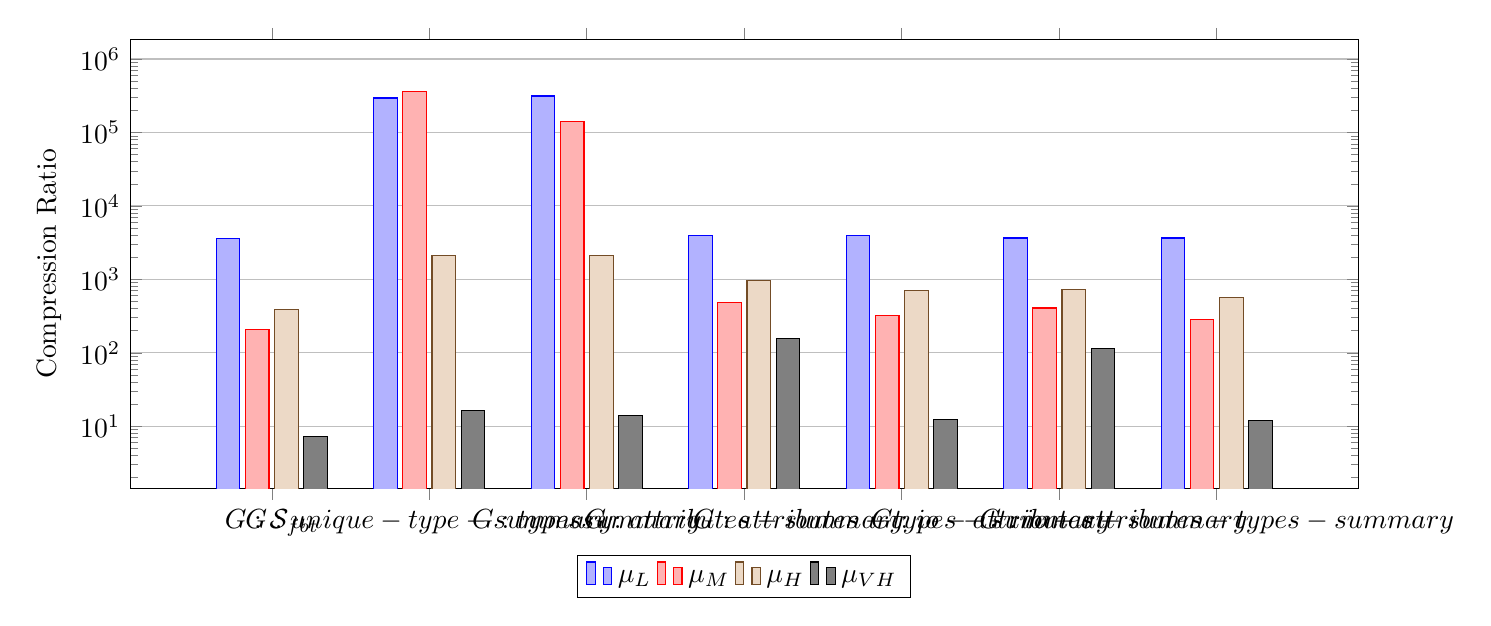
\begin{tikzpicture}
		\begin{axis}[
			ybar,
			symbolic x coords={$G:\mathcal{S}_{fbt}$,$G:\glssymbol{unique-type-summary}$,$G:\glssymbol{typessummary}$,$G:\glssymbol{attributes-summary}$,$G:\glssymbol{attributes-types-summary}$,$G:\glssymbol{io-attributes-summary}$,$G:\glssymbol{io-attributes-types-summary}$},
			enlargelimits=0.15,
			ylabel={Compression Ratio},
			x=2cm,
			bar width=0.3cm,
			xtick=data,
			ymode = log,
			ymajorgrids = true,
			legend style={at={(0.5,-0.15)},
			anchor=north,legend columns=-1},
		]
		\addplot coordinates {
			($G:\mathcal{S}_{fbt}$, 3589.49)
			($G:\glssymbol{unique-type-summary}$, 294067.89)
			($G:\glssymbol{typessummary}$, 313917.10)
			($G:\glssymbol{attributes-summary}$, 3999.70)
			($G:\glssymbol{attributes-types-summary}$, 3999.69)
			($G:\glssymbol{io-attributes-summary}$, 3654.78)
			($G:\glssymbol{io-attributes-types-summary}$, 3654.77)
		};

		\addplot coordinates {
			($G:\mathcal{S}_{fbt}$, 205.80)
			($G:\glssymbol{unique-type-summary}$, 361299.27)
			($G:\glssymbol{typessummary}$, 141978.05)
			($G:\glssymbol{attributes-summary}$, 490.00)
			($G:\glssymbol{attributes-types-summary}$, 326.39)
			($G:\glssymbol{io-attributes-summary}$, 407.85)
			($G:\glssymbol{io-attributes-types-summary}$, 283.95)
		};

		\addplot coordinates {
			($G:\mathcal{S}_{fbt}$, 386.79)
			($G:\glssymbol{unique-type-summary}$, 2103.26)
			($G:\glssymbol{typessummary}$, 2128.70)
			($G:\glssymbol{attributes-summary}$, 959.60)
			($G:\glssymbol{attributes-types-summary}$, 710.87)
			($G:\glssymbol{io-attributes-summary}$, 717.87)
			($G:\glssymbol{io-attributes-types-summary}$, 572.57)
		};

		\addplot coordinates {
			($G:\mathcal{S}_{fbt}$, 7.29)
			($G:\glssymbol{unique-type-summary}$, 16.21)
			($G:\glssymbol{typessummary}$, 14.08)
			($G:\glssymbol{attributes-summary}$, 154.86)
			($G:\glssymbol{attributes-types-summary}$, 12.34)
			($G:\glssymbol{io-attributes-summary}$, 113.75)
			($G:\glssymbol{io-attributes-types-summary}$, 12.04)
		};
		\legend{$\mu_L$,$\mu_M$,$\mu_H$,$\mu_{VH}$}
		\end{axis}
		\end{tikzpicture}
	}
	\caption{Compression ratio $G:\mathcal{S}$ of graph summaries. The ratio axis is reported in logarithmic scale.}
	\label{fig:vol-ration-bar}
\end{figure}

%\begin{figure}
%	\centering
%	\resizebox{\textwidth}{!}{
%		\begin{tikzpicture}
%		\begin{axis}[
%		ybar,
%		symbolic x coords={\glssymbol{unique-type-summary},\glssymbol{typessummary},\glssymbol{attributes-summary},\glssymbol{attributes-types-summary},\glssymbol{io-attributes-summary},\glssymbol{io-attributes-types-summary}},
%		enlargelimits=0.15,
%		ylabel={Compression Ratio},
%		x=2cm,
%		bar width=0.3cm,
%		xtick=data,
%		legend style={at={(0.5,-0.15)},
%			anchor=north,legend columns=-1},
%		]
%		\addplot coordinates {
%			(\glssymbol{unique-type-summary},1.89)
%			(\glssymbol{typessummary},1.77)
%			(\glssymbol{attributes-summary},81.73)
%			(\glssymbol{attributes-types-summary},81.74)
%			(\glssymbol{io-attributes-summary},89.57)
%			(\glssymbol{io-attributes-types-summary},89.57)
%		};
%
%		\addplot coordinates {
%			(\glssymbol{unique-type-summary},0.23)
%			(\glssymbol{typessummary},0.22)
%			(\glssymbol{attributes-summary},42.51)
%			(\glssymbol{attributes-types-summary},53.37)
%			(\glssymbol{io-attributes-summary},51.45)
%			(\glssymbol{io-attributes-types-summary},62.68)
%		};
%
%		\addplot coordinates {
%			(\glssymbol{unique-type-summary}, 17.81)
%			(\glssymbol{typessummary},17.60)
%			(\glssymbol{attributes-summary},47.99)
%			(\glssymbol{attributes-types-summary},62.55)
%			(\glssymbol{io-attributes-summary},66.13)
%			(\glssymbol{io-attributes-types-summary},79.45)
%		};
%
%		\addplot coordinates {
%			(\glssymbol{unique-type-summary}, 45.00)
%			(\glssymbol{typessummary},51.81)
%			(\glssymbol{attributes-summary},4.71)
%			(\glssymbol{attributes-types-summary},59.10)
%			(\glssymbol{io-attributes-summary},6.41)
%			(\glssymbol{io-attributes-types-summary},60.56)
%		};
%		\legend{$\mu_L$,$\mu_M$,$\mu_H$,$\mu_{VH}$}
%		\end{axis}
%		\end{tikzpicture}
%	}
%	\caption{Compression ratio of graph summaries}
%	\label{fig:vol-ration-bar}
%\end{figure}


\subsubsection{Performance of the Summarisation Relation}

Figure~\ref{fig:cpu-time-bar} depicts the average CPU time in $ms$ for each category of complexity. This time accounts for the \hyperref[step-he]{Step~3} (Section~\ref{chap03:algo:edge-materialisation}) in the graph summarisation computation.
For each dataset which raw data is reported in Table~\ref{tab:cpu-time}, the times are the average of two runs of a summarisation relation.

The \emph{unique type} $R_{ut}$ and types $R_t$ summarisation relations can have an undefined sumnode (Section~\ref{sec:undefined-sumnode}) due to some nodes having no type information. For performance reason, the undefined sumnode $\mathfrak{U}$ is filtered from the resulting summary. Therefore, reported run times in Table~\ref{tab:cpu-time} from $R_{ut}$ and $R_t$ cannot be compared to others.

On the \emph{Medium}, \emph{High}, and \emph{Very High} datasets, the time taken by the $R_{ut}$ summarisation on the \hyperref[step-he]{Step~3} of the graph summary computation is higher than $R_t$. This highlights the property of the $R_{ut}$ summarisation of being a many-to-many binary relation rather than a many-to-one, i.e., it can assign a node to several sumnodes. As a consequence, we need to compute all the possible combinations of edges between the sumnodes.
We note that the \gls{incoming-attributes} feature in $R_{ioa}$ and $R_{ioat}$ does not imply a higher runtime when compared to $R_{a}$ and $R_{at}$.

\begin{figure}
	\centering
	\resizebox{\textwidth}{!}{
		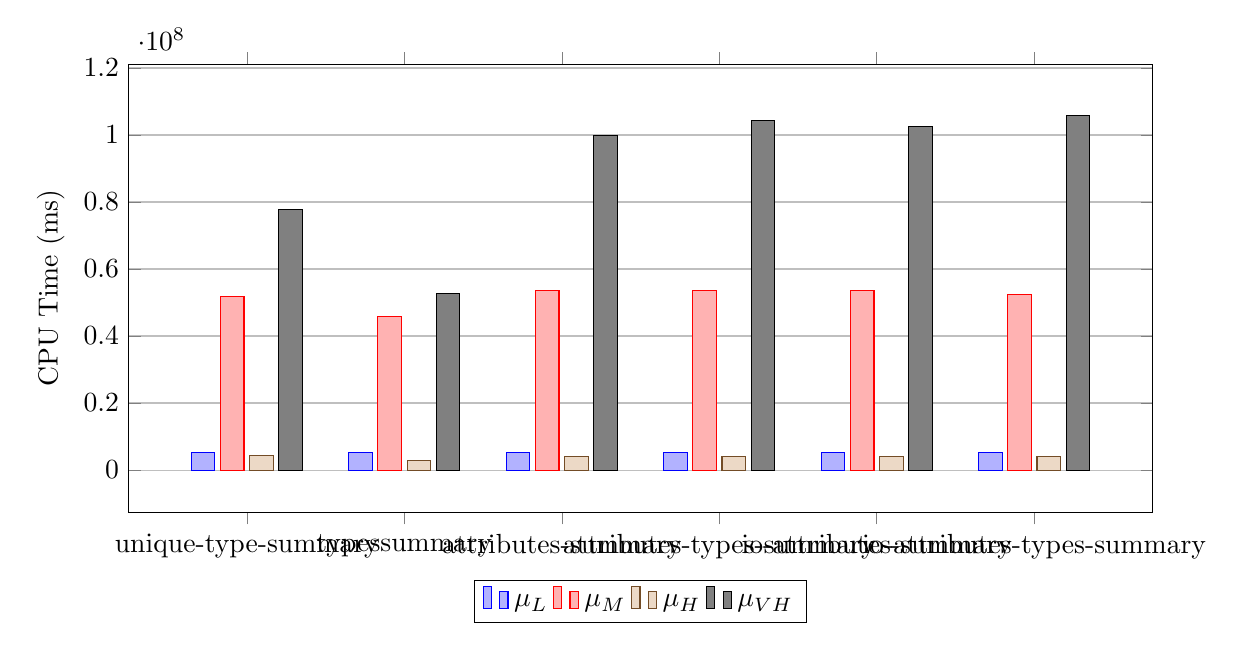
\begin{tikzpicture}
		\begin{axis}[
		compat=newest,
		ymajorgrids,
		ybar,
		symbolic x coords={\glssymbol{unique-type-summary},\glssymbol{typessummary},\glssymbol{attributes-summary},\glssymbol{attributes-types-summary},\glssymbol{io-attributes-summary},\glssymbol{io-attributes-types-summary}},
		enlargelimits=0.15,
		ylabel={CPU Time (ms)},
		x=2cm,
		bar width=0.3cm,
		xtick=data,
		legend style={at={(0.5,-0.15)},
			anchor=north,legend columns=-1},
		]
		\addplot coordinates {
			(\glssymbol{unique-type-summary}, 5181727)
			(\glssymbol{typessummary}, 5140988)
			(\glssymbol{attributes-summary}, 5208950)
			(\glssymbol{attributes-types-summary}, 5227250)
			(\glssymbol{io-attributes-summary}, 5254718)
			(\glssymbol{io-attributes-types-summary}, 5212401)
		};

		\addplot coordinates {
			(\glssymbol{unique-type-summary}, 51724125)
			(\glssymbol{typessummary}, 45942442)
			(\glssymbol{attributes-summary}, 53505035)
			(\glssymbol{attributes-types-summary}, 53487935)
			(\glssymbol{io-attributes-summary}, 53557640)
			(\glssymbol{io-attributes-types-summary}, 52440249)
		};

		\addplot coordinates {
			(\glssymbol{unique-type-summary}, 4246345)
			(\glssymbol{typessummary}, 2763572)
			(\glssymbol{attributes-summary}, 3962202)
			(\glssymbol{attributes-types-summary}, 3942577)
			(\glssymbol{io-attributes-summary}, 3989825)
			(\glssymbol{io-attributes-types-summary}, 4032795)
		};

		\addplot coordinates {
			(\glssymbol{unique-type-summary}, 77643685)
			(\glssymbol{typessummary}, 52608760)
			(\glssymbol{attributes-summary}, 99839325)
			(\glssymbol{attributes-types-summary}, 104255540)
			(\glssymbol{io-attributes-summary}, 102540080)
			(\glssymbol{io-attributes-types-summary}, 105685365)
		};

		\legend{$\mu_L$,$\mu_M$,$\mu_H$,$\mu_{VH}$}
		\end{axis}
		\end{tikzpicture}
	}
	\caption{Performance comparison of the graph summaries}
	\label{fig:cpu-time-bar}
\end{figure}


\subsubsection{Graph Summary Precision}

We discuss in this section the precision of a summary with regards to the \gls{connectivity} first, then to the \gls{type} and \gls{attribute} next. We do not report the precision in any error classification for the \texttt{dbpedia} dataset (Very High category). The reason is we were unable to evaluate the precision on it due to performance issues. While the performance evaluation did not account for the undefined sumnode $\mathfrak{U}$, we do consider it for the precision evaluation.

\minisec{Connectivity Precision}

Figure~\ref{fig:link-precision-bar} depicts the average connectivity precision for $P1$ and $P2$ over three categories of complexity, i.e., \emph{Low}, \emph{Medium}, and \emph{High}. The raw results for each dataset are reported in Table~\ref{tab:precision-conn} of the Appendix section; for each category of dataset complexity, we report as well the mean $\mu$ of the connectivity precision.\\

We discuss first the connectivity error with regards to the precision $P1$ plotted on Figure~\ref{fig:err-conn-p1}.
The \glspl{summarisation-relation} based only on the type feature, i.e., $R_{ut}$ and $R_t$, provide a low connectivity precision. Indeed, they show on average a connectivity precision of $25\%$ according to $P1$, i.e., $\mu_H=0.2414$ for the types summarisation relation $R_t$.

Summarisation based on the attribute feature only, i.e., the attributes summarisation relation $R_a$ , provide also a low precision on \emph{Medium} and \emph{High} categories. On the \emph{Low} category, the attribute feature exhibits a better precision than the type feature, i.e., $\mu_L=0.5579$ for $R_a$ against $\mu_H=0.3617$ for $R_{ut}$. However, when the type and attribute features are combined in the attributes \$ types summarisation relation $R_{at}$, this provides a significant increase of the precision across all three categories. According to $P1$, we reach on average a $50\%$ connectivity precision ($0.5124$) on the \emph{High} category for $R_{at}$, and at least $20\%$ on \emph{Medium}.

We remark that the incoming attribute in the IO attributes summarisation relation $R_{ioa}$ is an important feature that increases the precision. The $R_{ioa}$ summarisation provides a precision of $30\%$ on the \emph{Medium} up to $50\%$ on \emph{High}, whereas $R_a$ reaches $15\%$ on \emph{Medium} and $10\%$ on \emph{High}. Overall, we can achieve a good average connectivity precision with $R_{ioat}$ according to $P1$ when we add the type feature.\\

We remark that the overall precision $P2$ is very low on the datasets of \emph{Medium} and \emph{High} complexities. This suggests that few nodes of the summary have a high out-degree, creating a combinatorial explosion of false positive edges. This will be investigated in future work.

\begin{figure}
	\centering
	\begin{subfigure}{.8\textwidth}
		\centering
		\resizebox{\textwidth}{!}{
			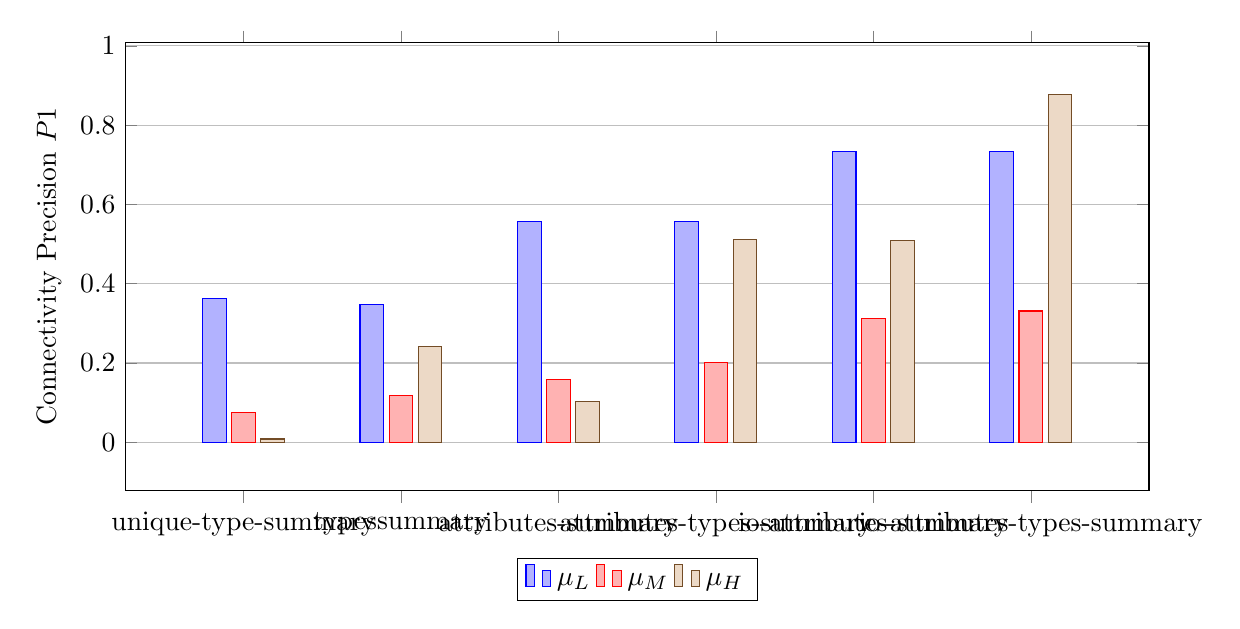
\begin{tikzpicture}
			\begin{axis}[
			compat=newest,
			ymajorgrids,
			ybar,
			symbolic x coords={\glssymbol{unique-type-summary},\glssymbol{typessummary},\glssymbol{attributes-summary},\glssymbol{attributes-types-summary},\glssymbol{io-attributes-summary},\glssymbol{io-attributes-types-summary}},
			enlargelimits=0.15,
			ylabel={Connectivity Precision $P1$},
			x=2cm,
			bar width=0.3cm,
			xtick=data,
			legend style={at={(0.5,-0.15)},
				anchor=north,legend columns=-1},
			]
			\addplot coordinates {
				(\glssymbol{unique-type-summary}, 0.3617)
				(\glssymbol{typessummary}, 0.3464)
				(\glssymbol{attributes-summary}, 0.5579)
				(\glssymbol{attributes-types-summary}, 0.5579)
				(\glssymbol{io-attributes-summary}, 0.7328)
				(\glssymbol{io-attributes-types-summary}, 0.7328)
			};

			\addplot coordinates {
				(\glssymbol{unique-type-summary}, 0.0757)
				(\glssymbol{typessummary}, 0.1190)
				(\glssymbol{attributes-summary}, 0.1591)
				(\glssymbol{attributes-types-summary}, 0.2011)
				(\glssymbol{io-attributes-summary}, 0.3123)
				(\glssymbol{io-attributes-types-summary}, 0.3311)
			};

			\addplot coordinates {
				(\glssymbol{unique-type-summary}, 0.0083)
				(\glssymbol{typessummary}, 0.2414)
				(\glssymbol{attributes-summary}, 0.1038)
				(\glssymbol{attributes-types-summary}, 0.5124)
				(\glssymbol{io-attributes-summary}, 0.5090)
				(\glssymbol{io-attributes-types-summary}, 0.8781)
			};
			\legend{$\mu_L$,$\mu_M$,$\mu_H$}
			\end{axis}
			\end{tikzpicture}
		}
		\caption{Precision $P1$}
		\label{fig:err-conn-p1}
	\end{subfigure}
	\quad
	\begin{subfigure}{.8\textwidth}
		\centering
		\resizebox{\textwidth}{!}{
			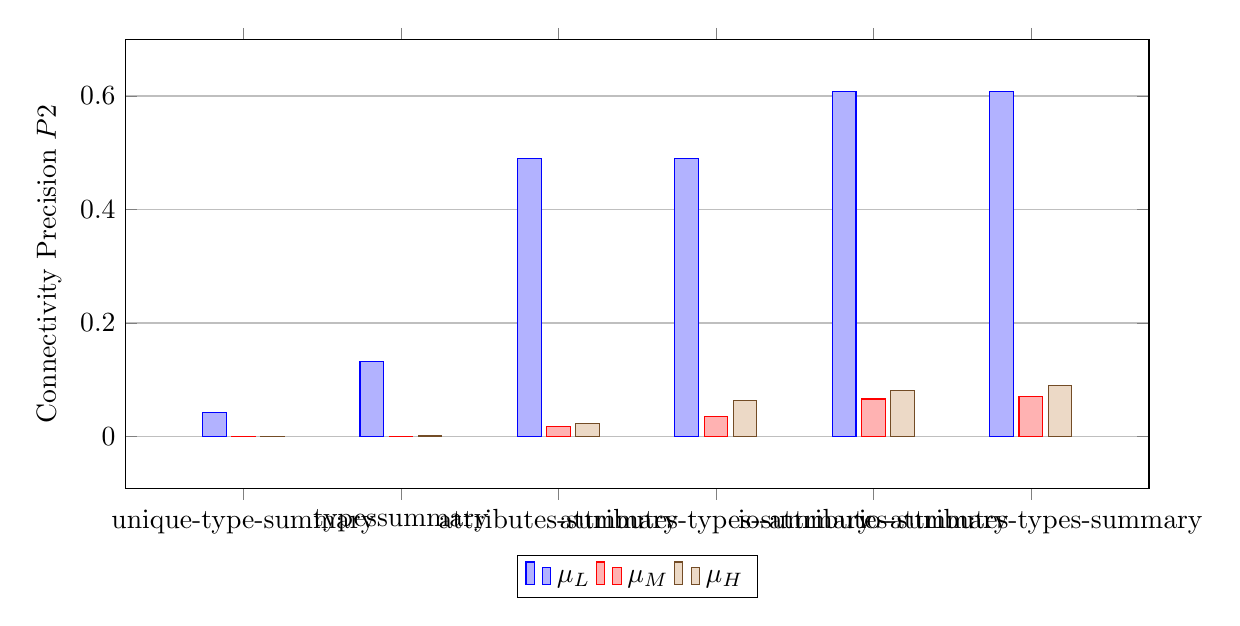
\begin{tikzpicture}
			\begin{axis}[
			compat=newest,
			ymajorgrids,
			ybar,
			symbolic x coords={\glssymbol{unique-type-summary},\glssymbol{typessummary},\glssymbol{attributes-summary},\glssymbol{attributes-types-summary},\glssymbol{io-attributes-summary},\glssymbol{io-attributes-types-summary}},
			enlargelimits=0.15,
			ylabel={Connectivity Precision $P2$},
			x=2cm,
			bar width=0.3cm,
			xtick=data,
			legend style={at={(0.5,-0.15)},
				anchor=north,legend columns=-1},
			]
			\addplot coordinates {
				(\glssymbol{unique-type-summary}, 0.0428)
				(\glssymbol{typessummary}, 0.1328)
				(\glssymbol{attributes-summary}, 0.4896)
				(\glssymbol{attributes-types-summary}, 0.4896)
				(\glssymbol{io-attributes-summary}, 0.6080)
				(\glssymbol{io-attributes-types-summary}, 0.6080)
			};

			\addplot coordinates {
				(\glssymbol{unique-type-summary}, 0.0003)
				(\glssymbol{typessummary}, 0.0002)
				(\glssymbol{attributes-summary}, 0.0181)
				(\glssymbol{attributes-types-summary}, 0.0352)
				(\glssymbol{io-attributes-summary}, 0.0660)
				(\glssymbol{io-attributes-types-summary}, 0.0701)
			};

			\addplot coordinates {
				(\glssymbol{unique-type-summary}, 0.0004)
				(\glssymbol{typessummary}, 0.0024)
				(\glssymbol{attributes-summary}, 0.0229)
				(\glssymbol{attributes-types-summary}, 0.0640)
				(\glssymbol{io-attributes-summary}, 0.0808)
				(\glssymbol{io-attributes-types-summary}, 0.0896)
			};
			\legend{$\mu_L$,$\mu_M$,$\mu_H$}
			\end{axis}
			\end{tikzpicture}
		}
		\caption{Precision $P2$}
		\label{fig:err-conn-p2}
	\end{subfigure}
	\caption{\Gls{connectivity} precision bar chart}
	\label{fig:link-precision-bar}
\end{figure}


\minisec{Schema Precision}

Figure~\ref{fig:schema-precision-bar} depicts the average type and attribute precisions over the categories of complexity.
In red we represent the attribute schema error, and in blue the type schema error. Bars with north east lines pattern depict $\mu_{L}$, with dotted pattern $\mu_{M}$, and with north west lines $\mu_{H}$.
The raw data is reported in Table~\ref{tab:precision-schema} of the Appendix section.

The summarisation relations $R_{ut}$ and $R_t$ based on the type feature provide an attribute precision above at least $60\%$ for $P1$ ($\mu_M=0.5927$ for $\sim_{ut}$).
On the contrary, the attribute feature reports a good type precision, reaching on average at least $90\%$ for $R_a$, i.e., $P1=0.9222$ on the \emph{Medium} datasets.

\gls{incoming-attributes} do not increase much the type precision, since the type precision of $R_a$ stays on par with $R_{ioa}$. The $R_{at}$ relation provides a perfect summarisation of the graph schema. Again, the significant differences between $P1$ and $P2$ suggests one more time that few nodes of the summary contains a high out-degree, creating a combinatorial explosion of false positive edges.

\begin{figure}
	\centering
	\begin{subfigure}{.8\textwidth}
		\centering
		\resizebox{\textwidth}{!}{
			\begin{tikzpicture}
			\pgfplotsset{
				grid=major,
				xmajorgrids=false,
				ybar stacked, ymin=0, ymax=2, xtick=data,
				symbolic x coords={\glssymbol{unique-type-summary},\glssymbol{typessummary},\glssymbol{attributes-summary},\glssymbol{attributes-types-summary},\glssymbol{io-attributes-summary},\glssymbol{io-attributes-types-summary}},
				enlargelimits=0.2,
				ylabel={Schema Precision $P1$},
				x=2cm,
				xtick=data
			}
			\begin{axis}[bar shift=-16pt]
			\addplot[postaction={pattern=north east lines}, fill=blue!30, draw = blue] coordinates {
				(\glssymbol{unique-type-summary}, 1.0000)
				(\glssymbol{typessummary}, 1.0000)
				(\glssymbol{attributes-summary}, 0.9999)
				(\glssymbol{attributes-types-summary}, 1.0000)
				(\glssymbol{io-attributes-summary}, 0.9999)
				(\glssymbol{io-attributes-types-summary}, 1.0000)
			};

			\addplot[postaction={pattern=north east lines}, fill=red!30, draw = red] coordinates {
				(\glssymbol{unique-type-summary}, 0.7586)
				(\glssymbol{typessummary}, 0.7529)
				(\glssymbol{attributes-summary}, 1.0000)
				(\glssymbol{attributes-types-summary}, 1.0000)
				(\glssymbol{io-attributes-summary}, 1.0000)
				(\glssymbol{io-attributes-types-summary}, 1.0000)
			};

			\end{axis}
			\begin{axis}

			\addplot[postaction={pattern=dots}, fill=blue!30, draw = blue] coordinates {
				(\glssymbol{unique-type-summary}, 1.0000)
				(\glssymbol{typessummary}, 1.0000)
				(\glssymbol{attributes-summary}, 0.9222)
				(\glssymbol{attributes-types-summary}, 1.0000)
				(\glssymbol{io-attributes-summary}, 0.9415)
				(\glssymbol{io-attributes-types-summary}, 1.0000)
			};

			\addplot[postaction={pattern=dots}, fill=red!30, draw = red] coordinates {
				(\glssymbol{unique-type-summary}, 0.5927)
				(\glssymbol{typessummary}, 0.6607)
				(\glssymbol{attributes-summary}, 1.0000)
				(\glssymbol{attributes-types-summary}, 1.0000)
				(\glssymbol{io-attributes-summary}, 1.0000)
				(\glssymbol{io-attributes-types-summary}, 1.0000)
			};

			\end{axis}
			\begin{axis}[bar shift=16pt]

			\addplot[postaction={pattern=north west lines}, fill=blue!30, draw = blue] coordinates {
				(\glssymbol{unique-type-summary}, 1.0000)
				(\glssymbol{typessummary}, 1.0000)
				(\glssymbol{attributes-summary}, 0.9675)
				(\glssymbol{attributes-types-summary}, 1.0000)
				(\glssymbol{io-attributes-summary}, 0.9760)
				(\glssymbol{io-attributes-types-summary}, 1.0000)
			};

			\addplot[postaction={pattern=north west lines}, fill=red!30, draw = red] coordinates {
				(\glssymbol{unique-type-summary}, 0.7826)
				(\glssymbol{typessummary}, 0.9446)
				(\glssymbol{attributes-summary}, 1.0000)
				(\glssymbol{attributes-types-summary}, 1.0000)
				(\glssymbol{io-attributes-summary}, 1.0000)
				(\glssymbol{io-attributes-types-summary}, 1.0000)
			};

			\end{axis}
			\end{tikzpicture}
		}
		\caption{Precision $P1$}
	\end{subfigure}
	\quad
	\begin{subfigure}{.8\textwidth}
		\centering
		\resizebox{\textwidth}{!}{
			\begin{tikzpicture}
			\pgfplotsset{
				grid=major,
				xmajorgrids=false,
				ybar stacked, ymin=0, ymax=2, xtick=data,
				symbolic x coords={\glssymbol{unique-type-summary},\glssymbol{typessummary},\glssymbol{attributes-summary},\glssymbol{attributes-types-summary},\glssymbol{io-attributes-summary},\glssymbol{io-attributes-types-summary}},
				enlargelimits=0.2,
				ylabel={Schema Precision $P2$},
				x=2cm,
				xtick=data
			}
			\begin{axis}[bar shift=-16pt]

			\addplot[postaction={pattern=north east lines}, fill=blue!30, draw = blue] coordinates {
				(\glssymbol{unique-type-summary}, 1.0000)
				(\glssymbol{typessummary}, 1.0000)
				(\glssymbol{attributes-summary}, 0.9995)
				(\glssymbol{attributes-types-summary}, 1.0000)
				(\glssymbol{io-attributes-summary}, 0.9999)
				(\glssymbol{io-attributes-types-summary}, 1.0000)
			};

			\addplot[postaction={pattern=north east lines}, fill=red!30, draw = red] coordinates {
				(\glssymbol{unique-type-summary}, 0.5217)
				(\glssymbol{typessummary}, 0.4968)
				(\glssymbol{attributes-summary}, 1.0000)
				(\glssymbol{attributes-types-summary}, 1.0000)
				(\glssymbol{io-attributes-summary}, 1.0000)
				(\glssymbol{io-attributes-types-summary}, 1.0000)
			};

			\end{axis}
			\begin{axis}

			\addplot[postaction={pattern=dots}, fill=blue!30, draw = blue] coordinates {
				(\glssymbol{unique-type-summary}, 1.0000)
				(\glssymbol{typessummary}, 1.0000)
				(\glssymbol{attributes-summary}, 0.7136)
				(\glssymbol{attributes-types-summary}, 1.0000)
				(\glssymbol{io-attributes-summary}, 0.7753)
				(\glssymbol{io-attributes-types-summary}, 1.0000)
			};

			\addplot[postaction={pattern=dots}, fill=red!30, draw = red] coordinates {
				(\glssymbol{unique-type-summary}, 0.2798)
				(\glssymbol{typessummary}, 0.2925)
				(\glssymbol{attributes-summary}, 1.0000)
				(\glssymbol{attributes-types-summary}, 1.0000)
				(\glssymbol{io-attributes-summary}, 1.0000)
				(\glssymbol{io-attributes-types-summary}, 1.0000)
			};

			\end{axis}
			\begin{axis}[bar shift=16pt]

			\addplot[postaction={pattern=north west lines}, fill=blue!30, draw = blue] coordinates {
				(\glssymbol{unique-type-summary}, 1.0000)
				(\glssymbol{typessummary}, 1.0000)
				(\glssymbol{attributes-summary}, 0.1424)
				(\glssymbol{attributes-types-summary}, 1.0000)
				(\glssymbol{io-attributes-summary}, 0.2151)
				(\glssymbol{io-attributes-types-summary}, 1.0000)
			};

			\addplot[postaction={pattern=north west lines}, fill=red!30, draw = red] coordinates {
				(\glssymbol{unique-type-summary}, 0.0843)
				(\glssymbol{typessummary}, 0.2398)
				(\glssymbol{attributes-summary}, 1.0000)
				(\glssymbol{attributes-types-summary}, 1.0000)
				(\glssymbol{io-attributes-summary}, 1.0000)
				(\glssymbol{io-attributes-types-summary}, 1.0000)
			};

			\end{axis}
			\end{tikzpicture}
		}
		\caption{Precision $P2$}
	\end{subfigure}
	\caption[\Gls{schema} precision bar chart]{Schema precision bar chart. In red we show the attribute schema error, and in blue the type schema error. Bars with north east lines pattern depict $\mu_{L}$, with dotted pattern $\mu_{M}$, and with north west lines $\mu_{H}$.}
	\label{fig:schema-precision-bar}
\end{figure}


\minisec{Discussion}

In conclusion, we observe that a combination of both type and attribute features is necessary to achieve a good precision. The results show that taking \gls{incoming-attributes} as a feature of the \gls{summarisation-relation} is important for the connectivity precision, but not for the schema.

However, there is place for improvement for overall connectivity precision especially on certain datasets. We observe that the precision $P2$ leads to very low precision values which is caused by a few summary nodes with a high out-degree. This indicates that the model of $P2$ is not appropriate for measuring the precision of a summary in terms of connectivity and schema.

\subsubsection{Trade-Offs}

We report in Figure~\ref{fig:trade-conn-volume} the trade-off between the average connectivity precision and the average compression ratio across all datasets among all the relations. We can distinguish two groups of relations, the type-based \glspl{summarisation-relation}, i.e., the types $R_t$ and the \emph{unique type} $R_{ut}$ summarisation relation, and the attribute-based ones, i.e., the attributes relation $R_a$, the attributes \& types relation $R_{at}$, the IO attributes relation $R_{ioa}$, and the IO attributes \& types relation $R_{ioat}$.\\

The type-based relations provide the best compression ratio, but also the worst precision. In the attribute group, the compression ratio among relations is close to each others, but their precision differs greatly, with $R_{ioat}$ ahead.

This suggests that in terms of trade-off between connectivity precision and compression ratio, $R_{ioat}$ is the best candidate.\\

We report in Figure~\ref{fig:trade-schema-volume} the trade-off between the average schema precision and the average compression ratio across all datasets among all the relations. Again we can distinguish the same two groups. However, in the attribute group, the precision does not differ as much among the candidates, each one being either equal or very close to $1$. In the type group, the \emph{Types} summarisation relation $R_t$ provides a reasonable precision for a good compression ratio.

This suggests that if the precision is primordial, the \emph{Attributes \& Types} relation $R_{at}$ is the best candidate, providing a perfect schema precision for the best compression ratio. However, if the compression is primordial instead and that some imperfection can be tolerated, then the \emph{Types} summarisation relation $R_t$ is the best candidate.\\

We report in Figure~\ref{fig:trade-conn-cpu} (respectively, \ref{fig:trade-schema-cpu}) the trade-off between the average connectivity precision (respectively, average schema precision) and the average CPU time across all datasets among all the \glspl{summarisation-relation}. Among the attribute-based algorithms $R_a$, $R_{at}$, $R_{ioa}$ and $R_{ioat}$, the latter is the one that achieves the best runtime with the highest precision. Among the type-based algorithms, the \emph{Types} summarisation $R_t$ achieves a lower runtime and a higher precision than the \emph{Unique Type} relation $R_{ut}$.

If the schema precision is primordial and a low connectivity precision can be tolerated, the \emph{Types} summarisation $R_t$ is the best candidate as it provides a high schema precision, with the best CPU time. On the contrary, if the connectivity is primordial, the summarisation relation $R_{ioat}$ is the best candidate, but this at the cost of a longer runtime.

\begin{figure}
	\centering
	\begin{subfigure}[t]{0.46\textwidth}
		\resizebox{\textwidth}{!}{
			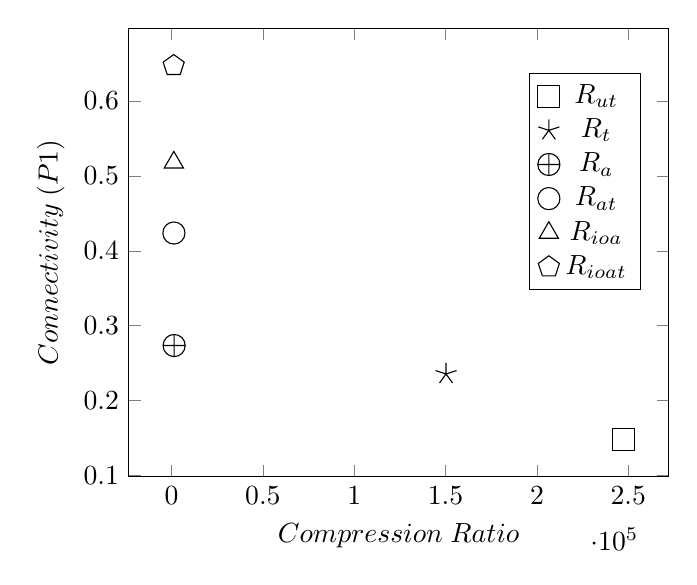
\begin{tikzpicture}
\begin{axis}[
  scatter/classes={
        a={mark=square},%
        b={mark=star},%
        c={mark=oplus},%
        d={mark=o},%
        e={mark=triangle},%
        f={mark=pentagon}
  },
  ylabel=$Connectivity \; (P1)$,
  xlabel=$Compression \; Ratio$,
  mark options={scale=2},
  legend style={at={(.95,0.9)}}
]
\addplot[scatter,only marks,scatter src=explicit symbolic]
coordinates {
% (6.6441, 0.14856667) [a] %0.1301) [a]
% (6.5291, 0.2356) [b] %0.2057) [b]
% (57.4105, 0.2736) [c] %0.2664) [c]
% (65.8846, 0.4238) [d] %0.4221) [d]
% (69.0500, 0.51803333) [e] %0.5169) [e]
% (77.2328, 0.64733333) [f] %0.6598) [f]

(247305.94, 0.14856667) [a]
(150252.41, 0.2356) [b]
(1433.53, 0.2736) [c]
(1314.50, 0.4238) [d]
(1268.24, 0.51803333) [e]
(1184.26, 0.64733333) [f]

};
\legend{$R_{ut}$, $R_{t}$, $R_{a}$, $R_{at}$, $R_{ioa}$, $R_{ioat}$}
\end{axis}
\end{tikzpicture}

		}
		\caption{Connectivity precision versus compression ratio.}
		\label{fig:trade-conn-volume}
	\end{subfigure}
	\qquad
	\begin{subfigure}[t]{0.46\textwidth}
		\resizebox{\textwidth}{!}{
			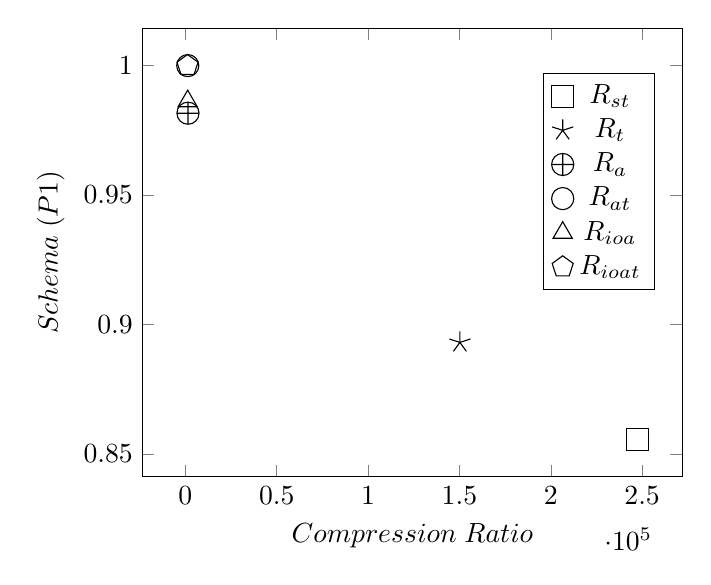
\begin{tikzpicture}
\begin{axis}[
  scatter/classes={
        a={mark=square},%
        b={mark=star},%
        c={mark=oplus},%
        d={mark=o},%
        e={mark=triangle},%
        f={mark=pentagon}
  },
  ylabel=$Schema \; (P1)$,
  xlabel=$Compression \; Ratio$,
  mark options={scale=2},
  legend style={at={(0.95,0.9)}}
]
\addplot[scatter,only marks,scatter src=explicit symbolic]
coordinates {
% (6.6441, 0.85565) [a] %0.6970) [a]
% (6.5291, 0.89303333) [b] %0.8585) [b]
% (57.4105, 0.9816) [c] %0.9733) [c]
% (65.8846, 1.0000) [d]
% (69.0500, 0.98623333) [e] %0.9795) [e]
% (77.2328, 1.0000) [f]

(247305.94, 0.85565) [a]
(150252.41, 0.89303333) [b]
(1433.53, 0.9816) [c]
(1314.50, 1.0000) [d]
(1268.24, 0.98623333) [e]
(1184.26, 1.0000) [f]

};
\legend{$R_{st}$, $R_{t}$, $R_{a}$, $R_{at}$, $R_{ioa}$, $R_{ioat}$}
\end{axis}
\end{tikzpicture}

		}
		\caption{Schema precision versus compression ratio.}
		\label{fig:trade-schema-volume}
	\end{subfigure}
	\qquad%
	\begin{subfigure}[t]{0.46\textwidth}
		\resizebox{\textwidth}{!}{
			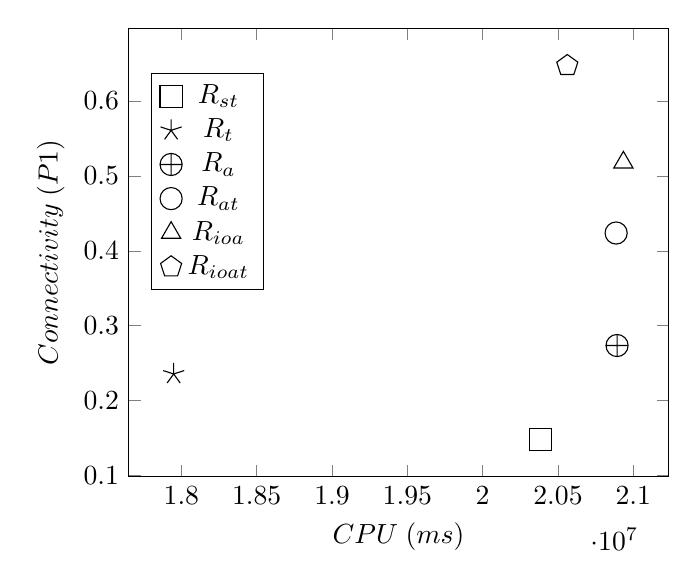
\begin{tikzpicture}
\begin{axis}[
  scatter/classes={
        a={mark=square},%
        b={mark=star},%
        c={mark=oplus},%
        d={mark=o},%
        e={mark=triangle},%
        f={mark=pentagon}
  },
  ylabel=$Connectivity \; (P1)$,
  xlabel=$CPU \; (ms)$,
  mark options={scale=2},
  legend style={at={(0.25,0.9)}}
]
\addplot[scatter,only marks,scatter src=explicit symbolic]
coordinates {
% (24844125.1190, 0.1301) [a]
% (24669863.0952, 0.2057) [b]
% (24277682.3810, 0.2664) [c]
% (28968841.4286, 0.4221) [d]
% (22053489.7619, 0.5169) [e]
% (22386809.1667, 0.6598) [f]
 (20384066, 0.14856667) [a]
 (17949001, 0.2356) [b]
 (20892062, 0.2736) [c]
 (20885921, 0.4238) [d]
 (20934061, 0.51803333) [e]
 (20561815, 0.64733333) [f]
};
\legend{$R_{st}$, $R_{t}$, $R_{a}$, $R_{at}$,
 $R_{ioa}$, $R_{ioat}$}
\end{axis}
\end{tikzpicture}

		}
		\caption{Connectivity precision versus summarisation performance.}
		\label{fig:trade-conn-cpu}
	\end{subfigure}
	\qquad%
	\begin{subfigure}[t]{0.46\textwidth}
		\resizebox{\textwidth}{!}{
			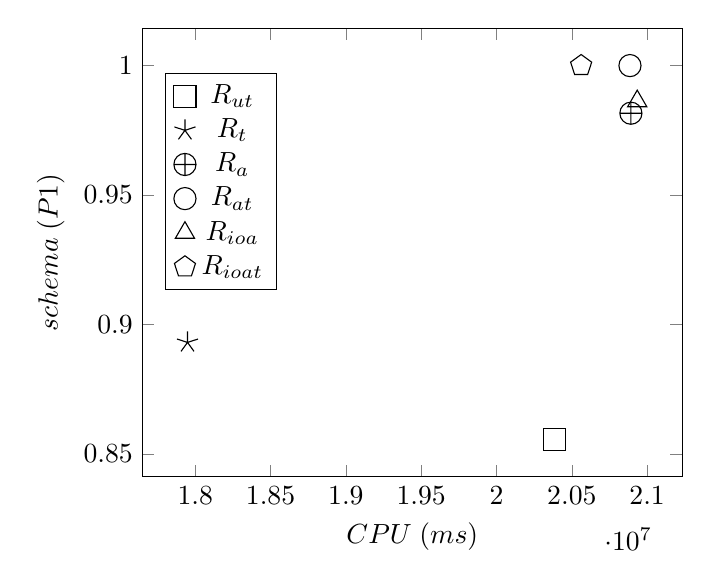
\begin{tikzpicture}
\begin{axis}[
  scatter/classes={
        a={mark=square},%
        b={mark=star},%
        c={mark=oplus},%
        d={mark=o},%
        e={mark=triangle},%
        f={mark=pentagon}
  },
  ylabel=$\gls{schema} \; (P1)$,
  xlabel=$CPU \; (ms)$,
  mark options={scale=2},
  legend style={at={(0.25,0.9)}}
]
\addplot[scatter,only marks,scatter src=explicit symbolic]
coordinates {
% (24844125.1190, 0.6970) [a]
% (24669863.0952, 0.8585) [b]
% (24277682.3810, 0.9733) [c]
%% (28968841.4286, 1.0000) [d]
% (22053489.7619, 0.9795) [e]
% (22386809.1667, 1.0000) [f]

 (20384066, 0.85565) [a]
 (17949001, 0.89303333) [b]
 (20892062, 0.9816) [c]
 (20885921, 1) [d]
 (20934061, 0.98623333) [e]
 (20561815, 1) [f]
};
\legend{$R_{ut}$, $R_{t}$, $R_{a}$, $R_{at}$, $R_{ioa}$, $R_{ioat}$}
\end{axis}
\end{tikzpicture}

		}
		\caption{Schema precision versus summarisation performance.}
		\label{fig:trade-schema-cpu}
	\end{subfigure}
	\caption{Efficiency and precision trade-offs of the candidate \glspl{summarisation-relation}. The values are taken as the average across all dataset categories.}
\end{figure}
